\documentclass[11pt, openright]{book}

	% Cover Variables
	\newcommand{\ctitle}{en pont monophasé}
	\newcommand{\cautor}{Lucas Lescure - Eva Maturana}
	\newcommand{\ctoptitle}{Commande MLI d'un onduleur}

	% Header Variables
		\newcommand{\headRE}{\emph{\thepage}}
		\newcommand{\headLE}{\emph{\thesection. \rightmark}}
		\newcommand{\footRE}{}
		\newcommand{\footLE}{}

	% TOC Variables
		\newcommand{\toctitle}{Table of Content}
		\newcommand{\tocchapter}{Chapter}
		\newcommand{\toccount}{3}
  
	% Chapter Variables
		\newcommand{\chvar}{Chapter -}

\usepackage[a4paper, total={16cm, 22.125cm}]{geometry}

% Page Style
\usepackage[]{environ}
% Cover Page 
\usepackage{tikz}
\makeatletter
\def\parsecomma#1,#2\endparsecomma{\def\page@x{#1}\def\page@y{#2}}
\tikzdeclarecoordinatesystem{page}{
    \parsecomma#1\endparsecomma
    \pgfpointanchor{current page}{north east}
    % Save the upper right corner
    \pgf@xc=\pgf@x%
    \pgf@yc=\pgf@y%
    % save the lower left corner
    \pgfpointanchor{current page}{south west}
    \pgf@xb=\pgf@x%
    \pgf@yb=\pgf@y%
    % Transform to the correct placement
    \pgfmathparse{(\pgf@xc-\pgf@xb)/2.*\page@x+(\pgf@xc+\pgf@xb)/2.}
    \expandafter\pgf@x\expandafter=\pgfmathresult pt
    \pgfmathparse{(\pgf@yc-\pgf@yb)/2.*\page@y+(\pgf@yc+\pgf@yb)/2.}
    \expandafter\pgf@y\expandafter=\pgfmathresult pt
}
\makeatother


% Object formatting
\usepackage[12pt]{moresize}
\usepackage[]{anyfontsize}
\usepackage{titlesec}
\usepackage{import}
\usepackage{floatrow}
\usepackage{enumitem}
\usepackage{changepage}
\usepackage[normalem]{ulem}
\usepackage{array}
\newcommand{\ul}[1]{\underline{#1}}

\usepackage[]{chngcntr}
\usepackage{ifthen}
\ifthenelse{\figcountdepth > 1}
  {\counterwithin{figure}{section}\counterwithin{table}{section}}
  {}

\usepackage[format=plain, labelfont=it, textfont=it]{caption}
\makeatletter
\def\@makecaption#1#2{%
    \vskip\abovecaptionskip
    \sbox\@tempboxa{\textit{#1.} #2}

       
   

    \ifdim \wd\@tempboxa >\hsize
        #1. #2\par
    \else
        \global \@minipagefalse
        \hb@xt@\hsize{\hfil\box\@tempboxa\hfil}
    \fi
    \vskip\belowcaptionskip}
\makeatother

\DeclareCaptionFormat{underline}{\uline{#1#2#3}\par}

% Sections
\titleformat{\section}{\fontsize{16}{19.2}\bfseries}{\thesection.}{0.25em}{}
\titleformat{\subsection}{\fontsize{14}{16.8}\bfseries}{\tab\thesubsection.}{0.25em}{}
\titleformat{\subsubsection}{\fontsize{10}{12}}{\uline{\thesubsubsection)\enspace}}{0em}{\uline}





% Geometry

% Typewritting

\setlength{\parskip}{1em}
\setlength{\parindent}{0em}


\newenvironment{items}[3][0pt]
{\def\closesep{#3}
    \vspace{#2}
    \begin{itemize}
        \setlength{\itemsep}{#1}
        \setlength{\topsep}{0pt}
        \setlength{\partopsep}{0pt}}
        {\end{itemize}
    \vspace{\closesep}}

\newenvironment{enum}[3][0pt]
{\defclosesep{#3}
    \vspace{#2}
    \begin{enumerate}
        \setlength{\itemsep}{#1}
        \setlength{\topsep}{0pt}
        \setlength{\partopsep}{0pt}}
        {\end{enumerate}
    \vspace{\closesep}}

\newenvironment{eq}[2]
{\def\closesep{#2}
    \vspace{#1}
    \begin{align*}}
        {\end{align*}
    \vspace{\closesep}}

\newenvironment{lfeq}[2]
{\def\closesep{#2}
    \vspace{#1}
    \begin{flalign*}}
        {\end{flalign*}
    \vspace{\closesep}}
% List Formatting


\NewEnviron{dent}[1]{
    \vspace{-10pt}
    \begin{adjustwidth}{7mm}{}
        \uline{#1}\hspace{2mm}
        \BODY
    \end{adjustwidth}
    \vspace{-10pt}
}


\usepackage[framemethod=tikz]{mdframed}
\newcounter{count_theorem}[section]\setcounter{count_theorem}{0}
\newcommand{\thetheorem}{\arabic{count_theorem}}

\newcounter{count_exercise}[section]\setcounter{count_exercise}{0}
\newcommand{\theexercise}{\arabic{count_exercise}}


\newenvironment{theorem}[1][]{
    \refstepcounter{count_theorem}
    \mdfsetup{
        linecolor=red!30,
        innerbottommargin=10pt,
        linewidth=2pt,
        topline=false,
        bottomline=false,
        rightline=false,
        shadow=true,
        shadowsize=4.5pt,
        frametitlerule=false,
        apptotikzsetting={
                \tikzset{
                    mdfbackground/.append style={
                            left color=red!8,right color=red!3
                        }
                }
            }
    }
    \begin{mdframed}[]\relax
        \ifstrempty{#1}
        {\textbf{Theorem~\thetheorem.} }
        {\textbf{Theorem~\thetheorem.~#1} }
        }
        {\end{mdframed}\vspace{-10pt}
}

\newenvironment{note}{
    \mdfsetup{innertopmargin=5pt,
        linecolor=gray!30,
        linewidth=2pt,
        topline=false,
        bottomline=false,
        rightline=false,
        frametitleaboveskip=0pt,
        shadow=false,
        shadowsize=4pt,
        frametitlerule=false,
        apptotikzsetting={
                \tikzset{
                    mdfbackground/.append style={
                            left color=gray!8,right color=gray!3
                        }
                }
            }
    }
    \begin{mdframed}[]\relax
        \textbf{Note. }
        }
        {\end{mdframed}\vspace{-10pt}
}

\newenvironment{example}{
    \mdfsetup{innertopmargin=5pt,
        linecolor=green!30,
        linewidth=2pt,
        topline=false,
        bottomline=false,
        rightline=false,
        frametitleaboveskip=0pt,
        shadow=false,
        shadowsize=4pt,
        frametitlerule=false,
        apptotikzsetting={
                \tikzset{
                    mdfbackground/.append style={
                            left color=green!7,right color=green!2
                        },
                    mdfframetitlebackground/.append style={
                            left color=green!7,right color=green!2
                        }
                }
            }
    }
    \begin{mdframed}[]\relax
        \textbf{Example. }
        }
        {\end{mdframed}\vspace{-10pt}
}


\usetikzlibrary{calc,arrows}

\tikzset{
    excursus arrow/.style={%
            line width=2pt,
            draw=gray!40,
            rounded corners=2ex,
        },
    excursus head/.style={
            fill=white,
            font=\bfseries\sffamily,
            text=gray!80,
            anchor=base west,
        },
    excursus line/.style={%
            line width=2pt,
            draw=gray!40,
            rounded corners=2ex,
        }
}

\newenvironment{exercise}[1][]{%
    \refstepcounter{count_exercise}
    \mdfsetup{
        singleextra={
                \path let \p1=(P), \p2=(O) in (\x2,\y1) coordinate (Q);
                \path let \p1=(Q), \p2=(O) in (\x1,{(\y1-\y2)/2}) coordinate (M);
                \path [excursus line] ($(O)+(5em,0ex)$) -| (M) |- ($(Q)+(20em,0ex)$);
                \node [excursus head] at ($(Q)+(2.5em,-0.75pt)$) {\ifstrempty{#1}{Exercise \theexercise}{Exercise \theexercise:~#1}};},
        firstextra={
                \path let \p1=(P), \p2=(O) in (\x2,\y1) coordinate (Q);
                \path [excursus arrow,-to] (O) |- ($(Q)+(12em,0ex)$) .. controls +(0:16em) and +(185:6em) .. ++(23em,2ex);},
        middlelinewidth=2.5em,middlelinecolor=white,
        hidealllines=true,topline=true,
        innertopmargin=0.5ex,
        innerbottommargin=2.5ex,
        innerrightmargin=2pt,
        innerleftmargin=2ex,
        skipabove=0.87\baselineskip,
        skipbelow=0.62\baselineskip,
    }
    \begin{mdframed}[]\relax}
        {\end{mdframed}\vspace{-10pt}
}

% Functions and Data Plotting
\usepackage{subfig,wrapfig,adjustbox,multirow}


% Plotting Style
\usepackage{graphicx,pgfplots}
\usetikzlibrary{arrows}
\usetikzlibrary {patterns,patterns.meta}
\usepgfplotslibrary{fillbetween}
\pgfplotsset{compat=1.18}

\usepgfplotslibrary{units}
% Logarithmic Scale
\pgfplotsset{
    log x ticks with fixed point/.style={
            xticklabel={
                    \pgfkeys{/pgf/fpu=true}
                    \pgfmathparse{exp(\tick)}%
                    \pgfmathprintnumber[fixed relative, precision=3]{\pgfmathresult}
                    \pgfkeys{/pgf/fpu=false}
                }
        }
}


\input{/root/.config/latex-utils/common/math.tex}

% Headings  
\usepackage[Glenn]{fncychap}
\ChNumVar{\fontsize{40}{42}}
\ChTitleVar{\Large\sc}
\ChNameVar{\Large\sc}
\setlength\headheight{14.5pt}
\renewcommand\FmN[1]{\chvar}



\usepackage{fancyhdr}
\usepackage{ragged2e}

% Header & Footers
\renewcommand{\chaptermark}[1]{\markboth{#1}{#1}}
\renewcommand{\sectionmark}[1]{
    \markright{ #1}
}
\pagestyle{fancy}
\fancyhf{}
\fancyhead[LE,RO]{\headLE}
\fancyhead[RE,LO]{\headRE}
\fancyfoot[LE,RO]{\footLE}
\fancyfoot[RE,LO]{\footRE}
\renewcommand{\headrulewidth}{0.5pt}
\fancyheadoffset{1cm}

\fancypagestyle{plain}{%
    \fancyhf{} % clear all header and footer fields
    \fancyfoot[LE, RO]{\footLE}
    \renewcommand{\headrulewidth}{0pt}
    \renewcommand{\footrulewidth}{0pt}}


\fancypagestyle{nohead}{%
    \fancyhf{} % clear all header 
    \fancyfoot[LE, RO]{\footLE}
    \fancyfoot[LO, RE]{\footRE}}

    \fancypagestyle{head}{%
    \fancyhf{} % clear all header 
    \fancyhead[LE,RO]{\headLE}
\fancyhead[RE,LO]{\headRE}
\renewcommand{\headrulewidth}{0.5pt}
\fancyheadoffset{1cm}
    }


\fancypagestyle{bib}{%
    \fancyhf{} % clear all header and footer fields
    \fancyhead[CE, CO]{}
    \fancyfoot[LE, RO]{\footLE}
    \fancyfoot[LO, RE]{Bibliographie}}

% Table of Contents

\renewcommand*\thechapter{\arabic{chapter}} %Usually Roman
\renewcommand*\thesection{\arabic{section}}
\renewcommand*\thesubsubsection{\thesubsection.\alph{subsubsection}}
\makeatletter
\@removefromreset{section}{chapter}
\makeatother


% Table of Contents

\usepackage{titletoc}
\usepackage[linktoc=all]{hyperref}
\addto{\captionsenglish}{\renewcommand*{\contentsname}{\toctitle}}

\setcounter{secnumdepth}{3}
\setcounter{tocdepth}{\toccount}

\usepackage[subfigure]{tocloft}
\setlength\cftparskip{0pt}

\usepackage{etoolbox}
\makeatletter
\pretocmd{\chapter}{\addtocontents{toc}{\protect\addvspace{5\p@}}}{}{}
\pretocmd{\section}{\addtocontents{toc}{\protect\addvspace{-10\p@}}}{}{}
\pretocmd{\subsection}{\addtocontents{toc}{\protect\addvspace{1\p@}}}{}{}
\makeatother


% Chapter Style
\titlecontents{chapter}
[11em]
{\bigskip}
{\bfseries\textsc\tocchapter~\textsc\thecontentslabel : \textsc}
{\hspace*{-5.5em}\textbf}
{\titlerule*[1pc]{ }}[\smallskip]

% Section Style
\titlecontents{section}
[3em] % i
{\bigskip\bfseries}
{\fontsize{11}{13.2}\bfseries\uline{\thecontentslabel.\enspace}\uline}
{\hspace*{-4em}\textbf}
{\hspace{-2mm}\uline{\hspace*{\fill}}\hspace{-5pt}\contentspage}

% Subsection Style
\titlecontents{subsection}
[5em] % i
{\smallskip\bfseries}
{\fontsize{10}{12}\bfseries\thecontentslabel.\enspace}
{\hspace*{-4em}}
{\titlerule*[0.5pc]{.}\contentspage}



% Subsubsection Style
\titlecontents{subsubsection}
[7em] % i
{\smallskip}
{\fontsize{10}{12}\thecontentslabel)\enspace}
{\hspace*{-4em}}
{\titlerule*[0.5pc]{.}\contentspage}











	% figure support
	\usepackage{import}
	\usepackage{xifthen}
	\pdfminorversion=7
	\usepackage{pdfpages}
	\usepackage{transparent}
	\newcommand{\incfig}[1]{%
			\def\svgwidth{\columnwidth}
			\import{./figures/}{#1.pdf_tex}
	}

	\pdfsuppresswarningpagegroup=1

\begin{document}
% Spacing
\input{/root/.config/latex-utils/common/begin.tex}

% Cover
% Cover
\definecolor{ccolor1}{RGB}{236,145,143}
\definecolor{ccolor2}{RGB}{131,168,192}
\definecolor{ccolor3}{RGB}{182,227,150}
\definecolor{ccolor4}{RGB}{171,206,145}

\begin{titlepage}

    \newgeometry{top=1cm, width=21cm, bottom=1cm}

    \begin{tikzpicture}[remember picture,overlay,every node/.style={anchor=center}]
        \node[opacity =0.07, inner sep=0pt, anchor=east] at (current page.east){\includegraphics[width=0.5\paperwidth,height=\paperheight]{/home/archlinux/.config/latex-utils/logos/invert1.png}};

        %\node[opacity=0.15, inner sep=0pt, anchor=south west] at (current page.south west){\includegraphics[width=0.5\paperwidth,height=0.5\paperheight]{/home/archlinux/.config/latex-utils/logos/invert2.png}};

        \node[opacity=0.15,inner sep=0pt, anchor=north west] at (current page.north west){\includegraphics[width=0.5\paperwidth,height=0.5\paperheight]{/home/archlinux/.config/latex-utils/logos/invert3.png}};

        \node at (page cs:0,0.925) {\LARGE\bfseries\textsc{Telecom Saint-Étienne}};


        %\node[opacity=0.15, inner sep=0pt, anchor=south west] at (current page.south west){\includegraphics[width=0.5\paperwidth,height=0.5\paperheight]{/home/archlinux/.config/latex-utils/logos/invert2.png}};

        \node at (page cs:0,0.6) {\fontsize{28}{28.8}\textbf{\ctoptitle}};
        \node at (page cs:0,0.525) {\fontsize{28}{28.8}\textbf{\ctitle}};
        \draw (page cs:0.5,0.475) -- (page cs:-0.5,0.475);
        \node at (page cs:0,0.445) {\Large\textsc{}};
        \node at (page cs:0,0.4) {\Large\textsc{\cdate}};
        \node[anchor=east] at (page cs:-0.3,0.315) {\Large\textsc{Lucas Lescure: }};
        \node[anchor=west] at (page cs:-0.3,0.335) {\Large\textsc{lucas.lescure1@gmail.com}};
        \node[anchor=west] at (page cs:-0.3,0.295) {\large\textsc{+33 6 16 06 04 45 / +34 638 57 83 09}};
        
        \node[anchor=east]  at (page cs:-0.3,0.255) {\Large\textsc{Aubin Sionville: }};
        \node[anchor=west]  at (page cs:-0.3,0.255) {\Large\textsc{aubin.sionville@telecom-st-etienne.fr}};

        \node[anchor=east]  at (page cs:-0.3,0.215) {\Large\textsc{Tom Paillet: }};
        \node[anchor=west]  at (page cs:-0.3,0.215) {\Large\textsc{tom.paillet@telecom-st-etienne.fr}};

        \node at (page cs:0,0.9) {\includegraphics[height=1.5cm]{/home/archlinux/.config/latex-utils/logos/Logo.png}\hspace{11cm}\includegraphics[height=1.5cm]{/home/archlinux/.config/latex-utils/logos/UJM.png}};

    \end{tikzpicture}

    % Telecom Logo Big
    \begin{tikzpicture}[remember picture,overlay,every node/.style={anchor=south west}]
        \fill[thin, fill=ccolor1, opacity=1] (page cs: -1,-0.39) arc (124.5:-4.7:10cm) -- (page cs: -1,-1) -- (page cs: -1,-0.39);
        \fill[thin, fill=ccolor2, opacity=1] (page cs: -1,-0.14) arc (92.3:53.25:10cm) arc (85.9:124.5:10cm) -- (page cs: -1,-0.14);
        \fill[thin, fill=ccolor3, opacity=1] (page cs: -1,-0.005) arc (106:18.7:10cm) arc(49:85.9:10cm) arc (53.25:92.3:10cm) -- (page cs: -1,-0.005);
        \fill[thin, fill=ccolor4, opacity=1] (page cs: -0.06,-1) arc (-16.65:52.5:10cm) arc (85.9:49:10cm) arc (18.7:-34:10cm) -- (page cs: -0.06,-1);
        \fill[thin, fill=white, opacity=1] (page cs: -0.17,-1) -- (page cs: -0.17,-0.523) -- (page cs: -0.525,-0.374) -- (page cs: -1,-0.57) -- (page cs: -1,-1) -- (page cs: -0.925,-1) -- (page cs: -0.925,-0.833) -- (page cs: -0.515,-0.665) -- (page cs: -0.515,-1) -- (page cs: -0.17,-1);
    \end{tikzpicture}
\end{titlepage}


\newgeometry{left=2.5cm, width=16cm, bottom=2cm, top=2cm}

\tikz[remember picture, overlay] \node[opacity=0.15,inner sep=0pt, anchor=north east] at (current page.north east){\includegraphics[angle=-90,origin=c,width=0.5\paperheight,height=0.5\paperwidth]{/home/archlinux/.config/latex-utils/logos/invert3.png}};
\tikz[remember picture,overlay] \node[opacity=0.15,inner sep=0pt, anchor=south east] at (current page.south east){\includegraphics[angle=90,width=0.5\paperwidth,height=0.5\paperheight]{/home/archlinux/.config/latex-utils/logos/invert2.png}};

\tableofcontents

\newgeometry{left=2.5cm, width=16cm, bottom=2.5cm, top=2.5cm}



\vspace{8.5cm}

\section*{Introduction}
\addcontentsline{toc}{subsection}{\hspace{2em}Introduction}

L'alimentation d'un moteur en courant alternative sinusoïdale est utile dans des application ou l'on souhaite un fonctionnement à vitesse constante. Ces sources sont typiquement fixées et donc pas adaptés pour des fonctionnement à vitesse variable. On préfèrera donc utiliser une commande MLI\footnote{Modulation en Largeur d'Impulsion}, permettant de controller la puissance fournie au moteur à partir d'une source continue de courant en faisant varier la largeur des impulsions.

Cependant lorsqu'une charge est alimenté par une commande MLI, il s'y présente des harmoniques sur le réseau qui nuisent la qualité de transfert de l'énergie, et interfèrent avec d'autres appareils sur le circuit. C'est pourquoi on cherchera donc comment supprimer les harmoniques multiples de rang $3$ et $5$ pour améliorer ce transfert d'énergie.


\newpage

\section{Objectifs du TP}

L'objectif de ce TP sera alors d'utiliser une structure en pont monophasé à IGBT\footnote{Insulated-Gate Bipolar Transistor} en commande MLI précalculée avec suppression des harmoniques $3$ et $5$.

\begin{figure}[ht!]
	\begin{tikzpicture}
		\node[overlay] at (-5,-3) {\includegraphics[width=0.6\textwidth]{./object/c1.png}};
		\draw[white] (-1.55,-1.4) -- (-5,-1.4);
		\draw[black!60, thin] (-6.55,-4.4) -- (-11,-4.4);
		\draw[black!60, thin] (-11,-4.4) -- (-11,-4.8) -- (-13,-4.8) -- (-13,-3.5) -- (-11,-3.5) -- (-11,-4.4);
		\node at(-12,-4.15) {\small Commande};
		\filldraw[fill=black] (-9.135,-4.4) circle (0.25mm);
		\node at (-5.75,-3.5) {\footnotesize$K_4$};
		\node at (-8.25,-3.5) {\footnotesize$K_3$};
		\node at (-5.75,-1.75) {\footnotesize$K_2$};
		\node at (-8.25,-1.75) {\footnotesize$K_1$};




	\end{tikzpicture}
	\caption{Structure en pont monophasé à IGBT}
\end{figure}

On rappelle aussi la forme d'onde de la tension de sortie qui est la suivante::

\begin{figure}[ht!]
	\centering
	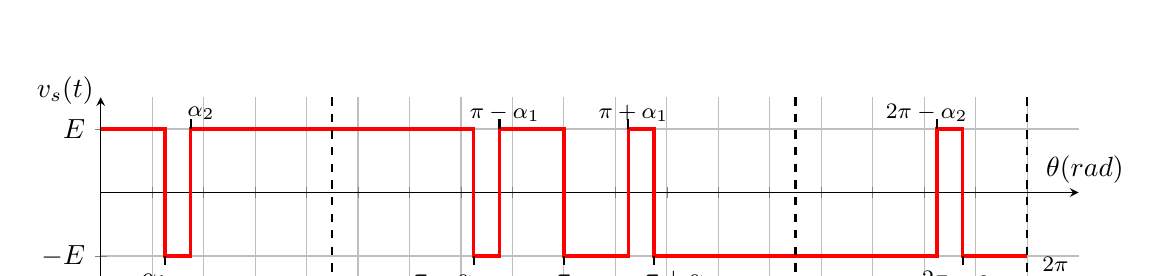
\begin{tikzpicture}
		\begin{axis}[
				width=14cm, height=4cm,
				xmin= 0, xmax= 19,
				ymin= -3, ymax = 3,
				xticklabels=\empty,yticklabels={ ,$-E$, , $E$},
				xtick={1,2,3,4,5,6,7,8,9,10,11,12,13,14,15,16,17,18},
				axis lines = middle,
				grid=both
			]
			\draw[red,very thick] (0,2) -- (1.25,2) -- (1.25,-2) -- (1.75,-2) -- (1.75,2) -- (7.25,2) -- (7.25,-2) -- (7.75, -2) -- (7.75,2) -- (9,2) -- (9,-2) -- (10.25,-2) -- (10.25,2) -- (10.75,2) -- (10.75,-2) -- (16.25,-2) -- (16.25,2) -- (16.75,2) -- (16.75,-2) -- (18,-2);
			\draw[thick] (1.25,-2) -- (1.25,-2.3);
			\node at (1.05,-2.75) {\footnotesize$\alpha_1$};
			\draw[thick] (1.75,2) -- (1.75,2.3);
			\node at (1.95,2.5){\footnotesize$\alpha_2$};
			\draw[thick] (7.25,-2) -- (7.25,-2.3);
			\node at (6.75,-2.75){\footnotesize$\pi-\alpha_2$};
			\draw[thick] (7.75,2) -- (7.75,2.3);
			\node at (7.85,2.5){\footnotesize$\pi-\alpha_1$};
			\draw[thick] (9,-2) -- (9,-2.3);
			\node at (9,-2.75){\footnotesize$\pi$};
			\draw[thick] (10.25,2) -- (10.25,2.3);
			\node at (10.35,2.5) {\footnotesize$\pi+\alpha_1$};
			\draw[thick] (10.75,-2) -- (10.75,-2.3);
			\node at (11.25,-2.75) {\footnotesize$\pi+\alpha_2$};
			\draw[thick] (16.75,-2) -- (16.75,-2.3);
			\node at (16.75,-2.75) {\footnotesize$2\pi-\alpha_1$};
			\draw[thick] (16.25,2) -- (16.25,2.3);
			\node at (16.05,2.5) {\footnotesize$2\pi-\alpha_2$};
			\draw[dashed,thick] (4.5,3) -- (4.5,-3);
			\draw[dashed,thick] (13.5,3) -- (13.5,-3);
			\draw[dashed,thick] (18,3) -- (18,-3);
			\node at (18.55,-2.25) {\footnotesize$2\pi$};
		\end{axis}
		\node at(-0.45,2.5) {$v_s(t)$};
		\node at(12.5,1.5) {$\theta(rad)$};
	\end{tikzpicture}
	\caption{Forme d'onde $v_s(t)$}
	\label{Forme d'onde $v_s(t)$}
\end{figure}

On utilisera, comme ci-présent sur la forme d'onde, $2$ degrés de liberté $\alpha_1$ et $\alpha_2$ qui permettrons la suppression des harmoniques sur le signal de commande MLI.

\subsection{Analyse spectrale du signal MLI}

D'après la Figure 1.2. on a :
\begin{items}{-15pt}{-15pt}
	\item $v_s(t)=-v_s(t)$: Donc c'est une fonction impaire et n'admet que des sinus dans le développement en série de Fourier de $v_s(t)$.
	\item $v_s\left( t+\frac{T}{2} \right) =-v_s(t)$: Donc il y a symétrie de de glissement et il n'y aura que des termes impaires dans la série de Fourier.
\end{items}
Ceci nous permet alors de réduire l'intervalle d'étude de la série de Fourier à $\ds{\frac{T}{4}}$, soit:
\begin{eq}{-10pt}{0pt}
	\widehat{V}_{s_{2k+1}}&=\frac{4E}{\pi}\left[ \int\limits_{0}^{\alpha_1} \sin\big((2k+1)\theta\big) \  d \theta - \int\limits_{\alpha_1}^{\alpha_2} \sin\big((2k+1)\theta\big) \  d \theta + \int\limits_{\alpha_2}^{\frac{\pi}{2}} \sin\big((2k+1)\theta\big) \  d \theta   \right]\\
	\widehat{V}_{s_{2k+1}}&=\frac{4E}{(2k+1)\pi}\Big[1-2\cos\big((2k+1)\alpha_1\big)+2\cos\big((2k+1)\alpha_2\big)\Big]
\end{eq}

On peut alors écrire:\\
$\ds{v_s(t)=\widehat{V}_{s_{2k+1}}\cdot \sin\big((2k+1)\omega t\big)}$\\
$\ds{v_s(t)=\frac{4E}{(2k+1)\pi}\Big[1-2\cos\big((2k+1)\alpha_1\big)+2\cos\big((2k+1)\alpha_2\big)\Big]\cdot \sin\big((2k+1)\omega t\big)}$

Ainsi pour trouver les valeurs de $\alpha_1$ et $\alpha_2$  afin d'éliminer les harmoniques $3$ et $5$ il suffit de résoudre le système : \\
\centerline{$\ds{\begin{cases}
				\widehat{V}_{s_3}=0=1-2\cos(3\alpha_1) + 2\cos(3\alpha_2) \\
				\widehat{V}_{s_1}=0=1-2\cos(5\alpha_1)+2\cos(5\alpha_2)
			\end{cases} \eqi \begin{cases}
				\alpha_1=23.6^{\circ} \\
				\alpha_2=33.3^{\circ}
			\end{cases}}$}

\subsection{Stratégie de commande}

En ce référant encore à la Figure 1.2. on peut établir la commande de l'onduleur en pont qui sera:
\begin{items}{-15pt}{-15pt}
	\item Pour $v_s=E$ alors les interrupteurs $K_1$ et $K_4$ doivent êtres ouvert donc $v_c=10\ V$.
	\item Pour $v_s=-E$ alors les interrupteurs $K_2$ et $K_3$ doivent êtres ouvert donc $v_c=0\ V$ (ou $-10\ V$) suivante le type de pont utilisé.
\end{items}

La commande devra donc avoir la forme suivante:

\begin{figure}[ht!]
	\centering
	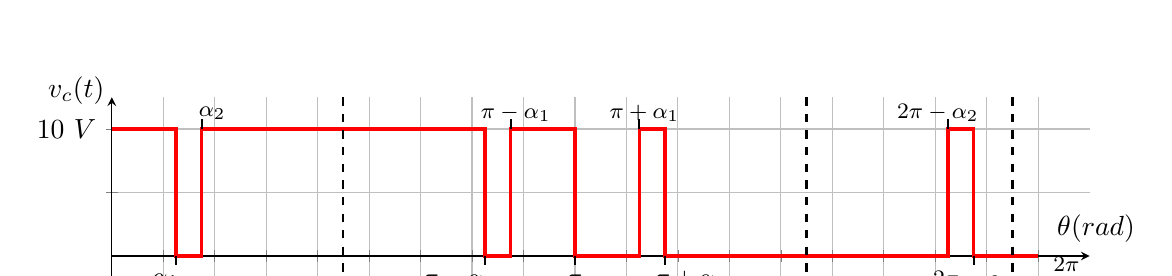
\begin{tikzpicture}
		\begin{axis}[
				width=14cm, height=4cm,
				xmin= 0, xmax= 19,
				ymin= -1, ymax = 5,
				xticklabels=\empty,yticklabels={ ,$0\ V$, , $10\ V$},
				xtick={1,2,3,4,5,6,7,8,9,10,11,12,13,14,15,16,17,18},
				axis lines = middle,
				grid=both
			]
			\draw[red,very thick] (0,4) -- (1.25,4) -- (1.25,0) -- (1.75,0) -- (1.75,4) -- (7.25,4) -- (7.25,0) -- (7.75, 0) -- (7.75,4) -- (9,4) -- (9,0) -- (10.25,0) -- (10.25,4) -- (10.75,4) -- (10.75,0) -- (16.25,0) -- (16.25,4) -- (16.75,4) -- (16.75,0) -- (18,0);
			\draw[thick] (1.25,0) -- (1.25,-0.3);
			\node at (1.05,-0.75) {\footnotesize$\alpha_1$};
			\draw[thick] (1.75,4) -- (1.75,4.3);
			\node at (1.95,4.5){\footnotesize$\alpha_2$};
			\draw[thick] (7.25,0) -- (7.25,-0.3);
			\node at (6.75,-0.75){\footnotesize$\pi-\alpha_2$};
			\draw[thick] (7.75,4) -- (7.75,4.3);
			\node at (7.85,4.5){\footnotesize$\pi-\alpha_1$};
			\draw[thick] (9,0) -- (9,-0.3);
			\node at (9,-0.75){\footnotesize$\pi$};
			\draw[thick] (10.25,4) -- (10.25,4.3);
			\node at (10.35,4.5) {\footnotesize$\pi+\alpha_1$};
			\draw[thick] (10.75,0) -- (10.75,-0.3);
			\node at (11.25,-0.75) {\footnotesize$\pi+\alpha_2$};
			\draw[thick] (16.75,0) -- (16.75,-0.3);
			\node at (16.75,-0.75) {\footnotesize$2\pi-\alpha_1$};
			\draw[thick] (16.25,4) -- (16.25,4.3);
			\node at (16.05,4.5) {\footnotesize$2\pi-\alpha_2$};
			\draw[dashed,thick] (4.5,5) -- (4.5,-1);
			\draw[dashed,thick] (13.5,5) -- (13.5,-1);
			\draw[dashed,thick] (17.5,5) -- (17.5,-1);
			\node at (18.55,-0.25) {\footnotesize$2\pi$};
		\end{axis}
		\node at(-0.45,2.5) {$v_c(t)$};
		\node at(12.5,0.75) {$\theta(rad)$};
	\end{tikzpicture}
	\caption{Forme d'onde de la commande $v_c(t)$}
	\label{Forme d'onde de la commande $v_c(t)$}
\end{figure}

Le schéma Synoptique de l'ensemble de la commande du convertisseur est la suivante:

\begin{figure}[ht]
	\begin{tikzpicture}
		\draw (0,0) -- (2,0) -- (2,1.5) -- (0,1.5) -- (0,0);
		\node at (1,0.75) {$\mu C$};
		\draw[-Latex] (2,1.2) -- (4,1.2);
		\draw[-Latex] (2,0.3) -- (4, 0.3);
		\draw (4,0) -- (6,0) -- (6,1.5) -- (4,1.5) -- (4,0);
		\node at (5,1) {\footnotesize Translateur};
		\node at (5,0.5) {\footnotesize de niveau};
		\draw[-Latex] (6,0.75) -- (8,0.75);
		\node at (9,1.2) {\footnotesize $v_c(t) = [0;\ 10V]$};
		\node at (8.5,0.75) {\footnotesize ou};
		\node at (9,0.3) {\footnotesize $v_c(t)=[-10V;\ 10V]$};

	\end{tikzpicture}
\end{figure}

\section{Pré-étude}

On peut découper le signal $v_s(t)$ comme une succession de signaux créneaux de période et durée à l'état haut variables. Cependant ces signaux ont chacun un $\alpha$ et $T$ différent comme on peut voir ci-dessous:

\begin{figure}[ht!]
	\centering
	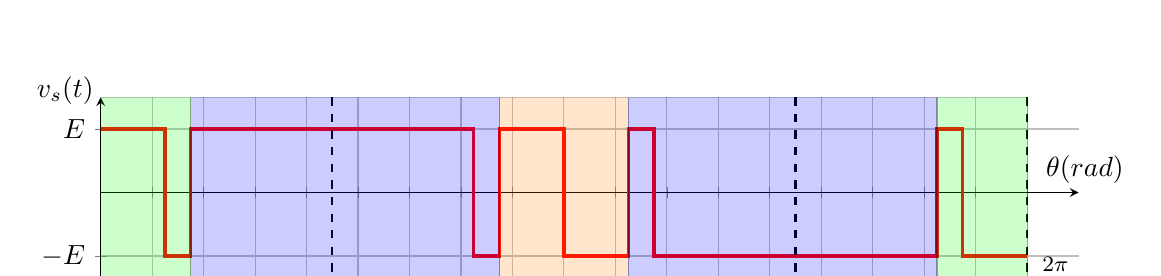
\begin{tikzpicture}
		\begin{axis}[
				width=14cm, height=4cm,
				xmin= 0, xmax= 19,
				ymin= -3, ymax = 3,
				xticklabels=\empty,yticklabels={ ,$-E$, , $E$},
				xtick={1,2,3,4,5,6,7,8,9,10,11,12,13,14,15,16,17,18},
				axis lines = middle,
				grid=both
			]
			\draw[red,very thick] (0,2) -- (1.25,2) -- (1.25,-2) -- (1.75,-2) -- (1.75,2) -- (7.25,2) -- (7.25,-2) -- (7.75, -2) -- (7.75,2) -- (9,2) -- (9,-2) -- (10.25,-2) -- (10.25,2) -- (10.75,2) -- (10.75,-2) -- (16.25,-2) -- (16.25,2) -- (16.75,2) -- (16.75,-2) -- (18,-2);
			\draw[dashed,thick] (4.5,3) -- (4.5,-3);
			\draw[dashed,thick] (13.5,3) -- (13.5,-3);
			\draw[dashed,thick] (18,3) -- (18,-3);
			\node at (18.55,-2.25) {\footnotesize$2\pi$};
			\filldraw[opacity=0.2, fill=green] (0,-3) -- (0,3) -- (1.75,3) -- (1.75,-3);
			\filldraw[opacity=0.2, fill=blue] (1.75,-3) -- (1.75,3) -- (7.75,3) -- (7.75,-3);
			\filldraw[opacity=0.2, fill=orange] (7.75,-3) -- (7.75,3) -- (10.25,3) -- (10.25,-3);
			\filldraw[opacity=0.2, fill=blue] (10.25,-3) -- (10.25,3) -- (16.25,3) -- (16.25,-3);
			\filldraw[opacity=0.2, fill=green] (16.25,-3) -- (16.25,3) -- (18,3) -- (18,-3);
		\end{axis}
		\node at(-0.45,2.5) {$v_s(t)$};
		\node at(12.5,1.5) {$\theta(rad)$};
	\end{tikzpicture}
	\caption{Forme d'onde $v_s(t)$ découpée en 5 créneaux}
\end{figure}

On peut relever ces signaux créneaux dans le tableau suivant avec $\Delta_k =\alpha'_k\cdot T_k$:
\begin{figure}[ht!]
	\begin{tabular}{|c|c|c|c|c|c|}
		\hline
		$\Delta_k$ & $\alpha_1$ & $\pi-2\alpha_2$         & $\alpha_1$  & $\alpha_2-\alpha_1$     & $\alpha_2-\alpha_1$ \\
		\hline
		$T_k$      & $\alpha_2$ & $\pi-\alpha_2-\alpha_1$ & $2\alpha_2$ & $\pi-\alpha_1-\alpha_2$ & $\alpha_2$          \\
		\hline
	\end{tabular}
\end{figure}

Pour des raison de commodité on choisira une horloge pour le PWM qui aura 36000 période d'horloge pour une période du PWM, soit $36000\ T_{clock}= T_{total}$. Ainsi pour un réseau de période $20\ ms$ ($50\ H_z$), on a une période d'horloge à $T_{clock}=55.5\ ns$ et de fréquence $f_{clock}=1.8\ MH_z$

\section{Réalisation}

\subsection{Assemblage}

On va réaliser la commande de l'onduleur à l'aide du logiciel PSoC\footnote{Programmable System-on-Chip} en utilisant la carte microcontrôlleur CY8CKIT-042 PSoC 4 Pioneer Kit du fabricant Inifneon sur laquel nous avons un chip CY8C4225AXI-483.

Sur un nouveau projet vide, on instancie le \texttt{PWM(TCPPWM mode)} dans la fenêtre \texttt{TopDesign}. On configure alors le composant en cochant \texttt{On terminal count} puis on insère dans la case \texttt{Period} la valeur de $T_1=\alpha_1 = 2360$, et dans la case \texttt{Compare} la valeur du rapport cyclique $\Delta_1=\alpha_2 = 3330$.

On ajoute de la même façon le composant \texttt{Clock} (renomée "clock"), en lui configurant une fréquence $f_{clock}=1.8\ MH_z$, le composant \texttt{Interrupt}(renomée "isr") et un \texttt{Digital Output Pin}(renomé "PWM\_OUT"). On relie ensuite ces composants par un fil au PWM avec le composant \texttt{Clock} allant vers l'entrée \texttt{clock}, le composant \texttt{Interrupt} branché à la sortie \texttt{interrupt}, et le \texttt{Digital Output Pin} à la sortie \texttt{line}.

\begin{figure}[ht!]
	\centering
	\includegraphics[width=0.4\textwidth]{./object/c2.png}
	\caption{Cablage des composant en \texttt{TopDesign} du projet}
\end{figure}

\subsection{Programmation}

On utilisera des variable globale dans le fichier \texttt{main.c} pour les durées à l'état haut et les périodes.Ainsi on fera intervenir dans des tableau \texttt{volatile}, \texttt{delta[5]} et \texttt{T[5]}, les valeurs précédemment trouvés lors de la pré-étude. Le qualificatif \texttt{volatile} est utilisé pour ne pas optimiser l'accès à la variable de façon à ce que le tableau puisse être utilisé par l'interruption même si une tache concurente l'utilisait.

On vas aussi définir des macros \texttt{alpha1},\texttt{alpha2} et \texttt{demip} pour remplacer la valeur de $\alpha_1$, $\alpha_2$ et celle de la demi période.

\begin{figure}[ht!]
	\centering
	\begin{tabular}{c}
		\begin{lstlisting}
#include "fonction.h"
			
#define alpha1 2360
#define alpha2 3330
#define demip 18000

volatile uint16_t delta[5]={alpha1, demip-2*alpha2, alpha1, alpha2-alpha1, alpha2-alpha1};
volatile uint16_t T[5]={alpha2, demip-alpha2-alpha1, 2*alpha1, demip-alpha1-alpha2, alpha2};
			\end{lstlisting}
	\end{tabular}
	\caption{Déclaration et initialisation des variables globales dans le \texttt{main.c}}
\end{figure}

Pour l'interruption on utilisera la fonction \texttt{isr\_StartEx()} qui prendra en paramètre le nom de notre interruption, ici \texttt{moninter}. On définira cette interruption dans le fichier \texttt{fonction.c} pour ceci on créé d'abord le fichier \texttt{fonction.h} dans lequel on utilise un API\footnote{Application Programming Interface} avec la libraire \texttt{project.h}. Grâce à celle ci on peut alors déclarer une interruption \texttt{moninter} de la façon suivante.

\begin{figure}[ht!]
	\centering
	\begin{tabular}{c}
		\begin{lstlisting}
#ifndef INTERRUPT_HEADER
	#define INTERRUPT_HEADER
	#include "project.h"
	void startup(void);
	CY_ISR_PROTO(moninter);
#endif
			\end{lstlisting}
	\end{tabular}
	\caption{Contenu du fichier \texttt{fonction.h}}
\end{figure}

On en profite aussi pour déclarer la fonction \texttt{startup()} qui permettra d'initialiser les périphériques au démarrage.

On code alors dans le fichier \texttt{fonction.c} les définitions des fonctions \texttt{startup()} et \texttt{CY\_ISR(moninter)} qui sera déclenchée dans l'évènement d'une interruption. Dans le cas de l'interruption on affecte à une variable globale \texttt{source}, la source de l'interruption en veillant à plus tard effacer cette source pour éviter de rentrer dans une boucle infinie.

Le NVIC\footnote{Nested Vector Interrupt Controller} gère les demandes d'interruption et les envois au processeur. Quand une interruption est déclenchée un signal est envoyé au NVIC pour executer l'interruption correspondante définie dans notre programme, à la fin de l'interruption il faut remettre ce signal à 0 pour eviter que le NVIC ne réexécute l'interruption, c'est pourquoi on fait intervenir la fonction \texttt{PWM\_ClearInterrupt()} qui éfface la source d'interruption au NVIC.

Pour récupérer la source on utilise une variable globale \texttt{source} à laquelle on lui affecte la valeur de l'interruption avec la commande \texttt{GetInterruptSourceMasked()} pour qu'elle puisse ensuite être gérée par le NVIC dans la commande \texttt{PWM\_ClearInterrupt(source)}.

Dans l'interruption on affecte les valeurs de \texttt{Compare} et \texttt{Period} du MLI en utilisant les tableaux définis dans le fichier \texttt{main.c} donc il faut utiliser le mot clé \texttt{extern} pour que l'interruption puisse les accéder.

Cette affectation doit être réalisé à chaque coup d'interruption c'est à dire à chaque fois que la période d'un créneaux est finie. Pour passer d'un créneau à l'autre on définis une variable locale \texttt{i} à l'aide du mot clé \texttt{static} et qui permettra à la variable de réserver en emplacement mémoire qui ne sera pas désallouée quand le compilateur sort de l'interruption. On évite ainsi une erreur de segmentation car sans ce mot clé, la mémoire sera désallouée mais à la prochaine interruption on réutilise cette variable qui a déjà été définie mais qui n'as plus d'emplacement mémoire.

\begin{figure}[ht!]
	\centering
	\begin{tabular}{c}
		\begin{lstlisting}
#include "fonction.h"
extern uint16_t delta[5];
extern uint16_t T[5];

void startup () {
	Clock_Start();
	PWM_Start();
	isr_StartEx(moninter);
}

CY_ISR(moninter) {
	// Declaration de la variable source d'interruption
	uint32 source;
	//Affectation de la source d'interruption a la variable source
	source = GetInterruptSourceMasked();
	//Code a inserer
	static volatile uint8_t i=0;
	i = (i + 1) % 5;
	//Utilisation des fonctions PWM_WritePeriod() et PWM_WriteCompare()
	PWM_WriteCompare(delta[i]);
	PWM_WritePeriod(T[i]);
	//Effacage de la source d'interruption pour eviter la boucle infinie
	PWM_ClearInterrupt(source);
}
			\end{lstlisting}
	\end{tabular}
	\caption{Contenu du fichier \texttt{fonction.c}}
\end{figure}

\begin{figure}[ht!]
	\hspace{-3.5cm}
	\begin{tabular}{c}
		\begin{lstlisting}
int main() {
	CyGlobalIntEnable //Enable global interrupts

	//Place your initialisation/startup code here
	startup();

	for(;;) {
		//Place your application code here
	}
}
			\end{lstlisting}
	\end{tabular}
	\caption{Contenu du main dans le fichier \texttt{main.c}}
\end{figure}


\newpage
\subsection{Mise en Pratique}

On effectue le teste en utilisant un oscilloscope ayant le module FFT pour obtenir le spectre du signal de sortie du bloc MLI.
\begin{figure}[ht!]
	\begin{floatrow}
		\ffigbox{
			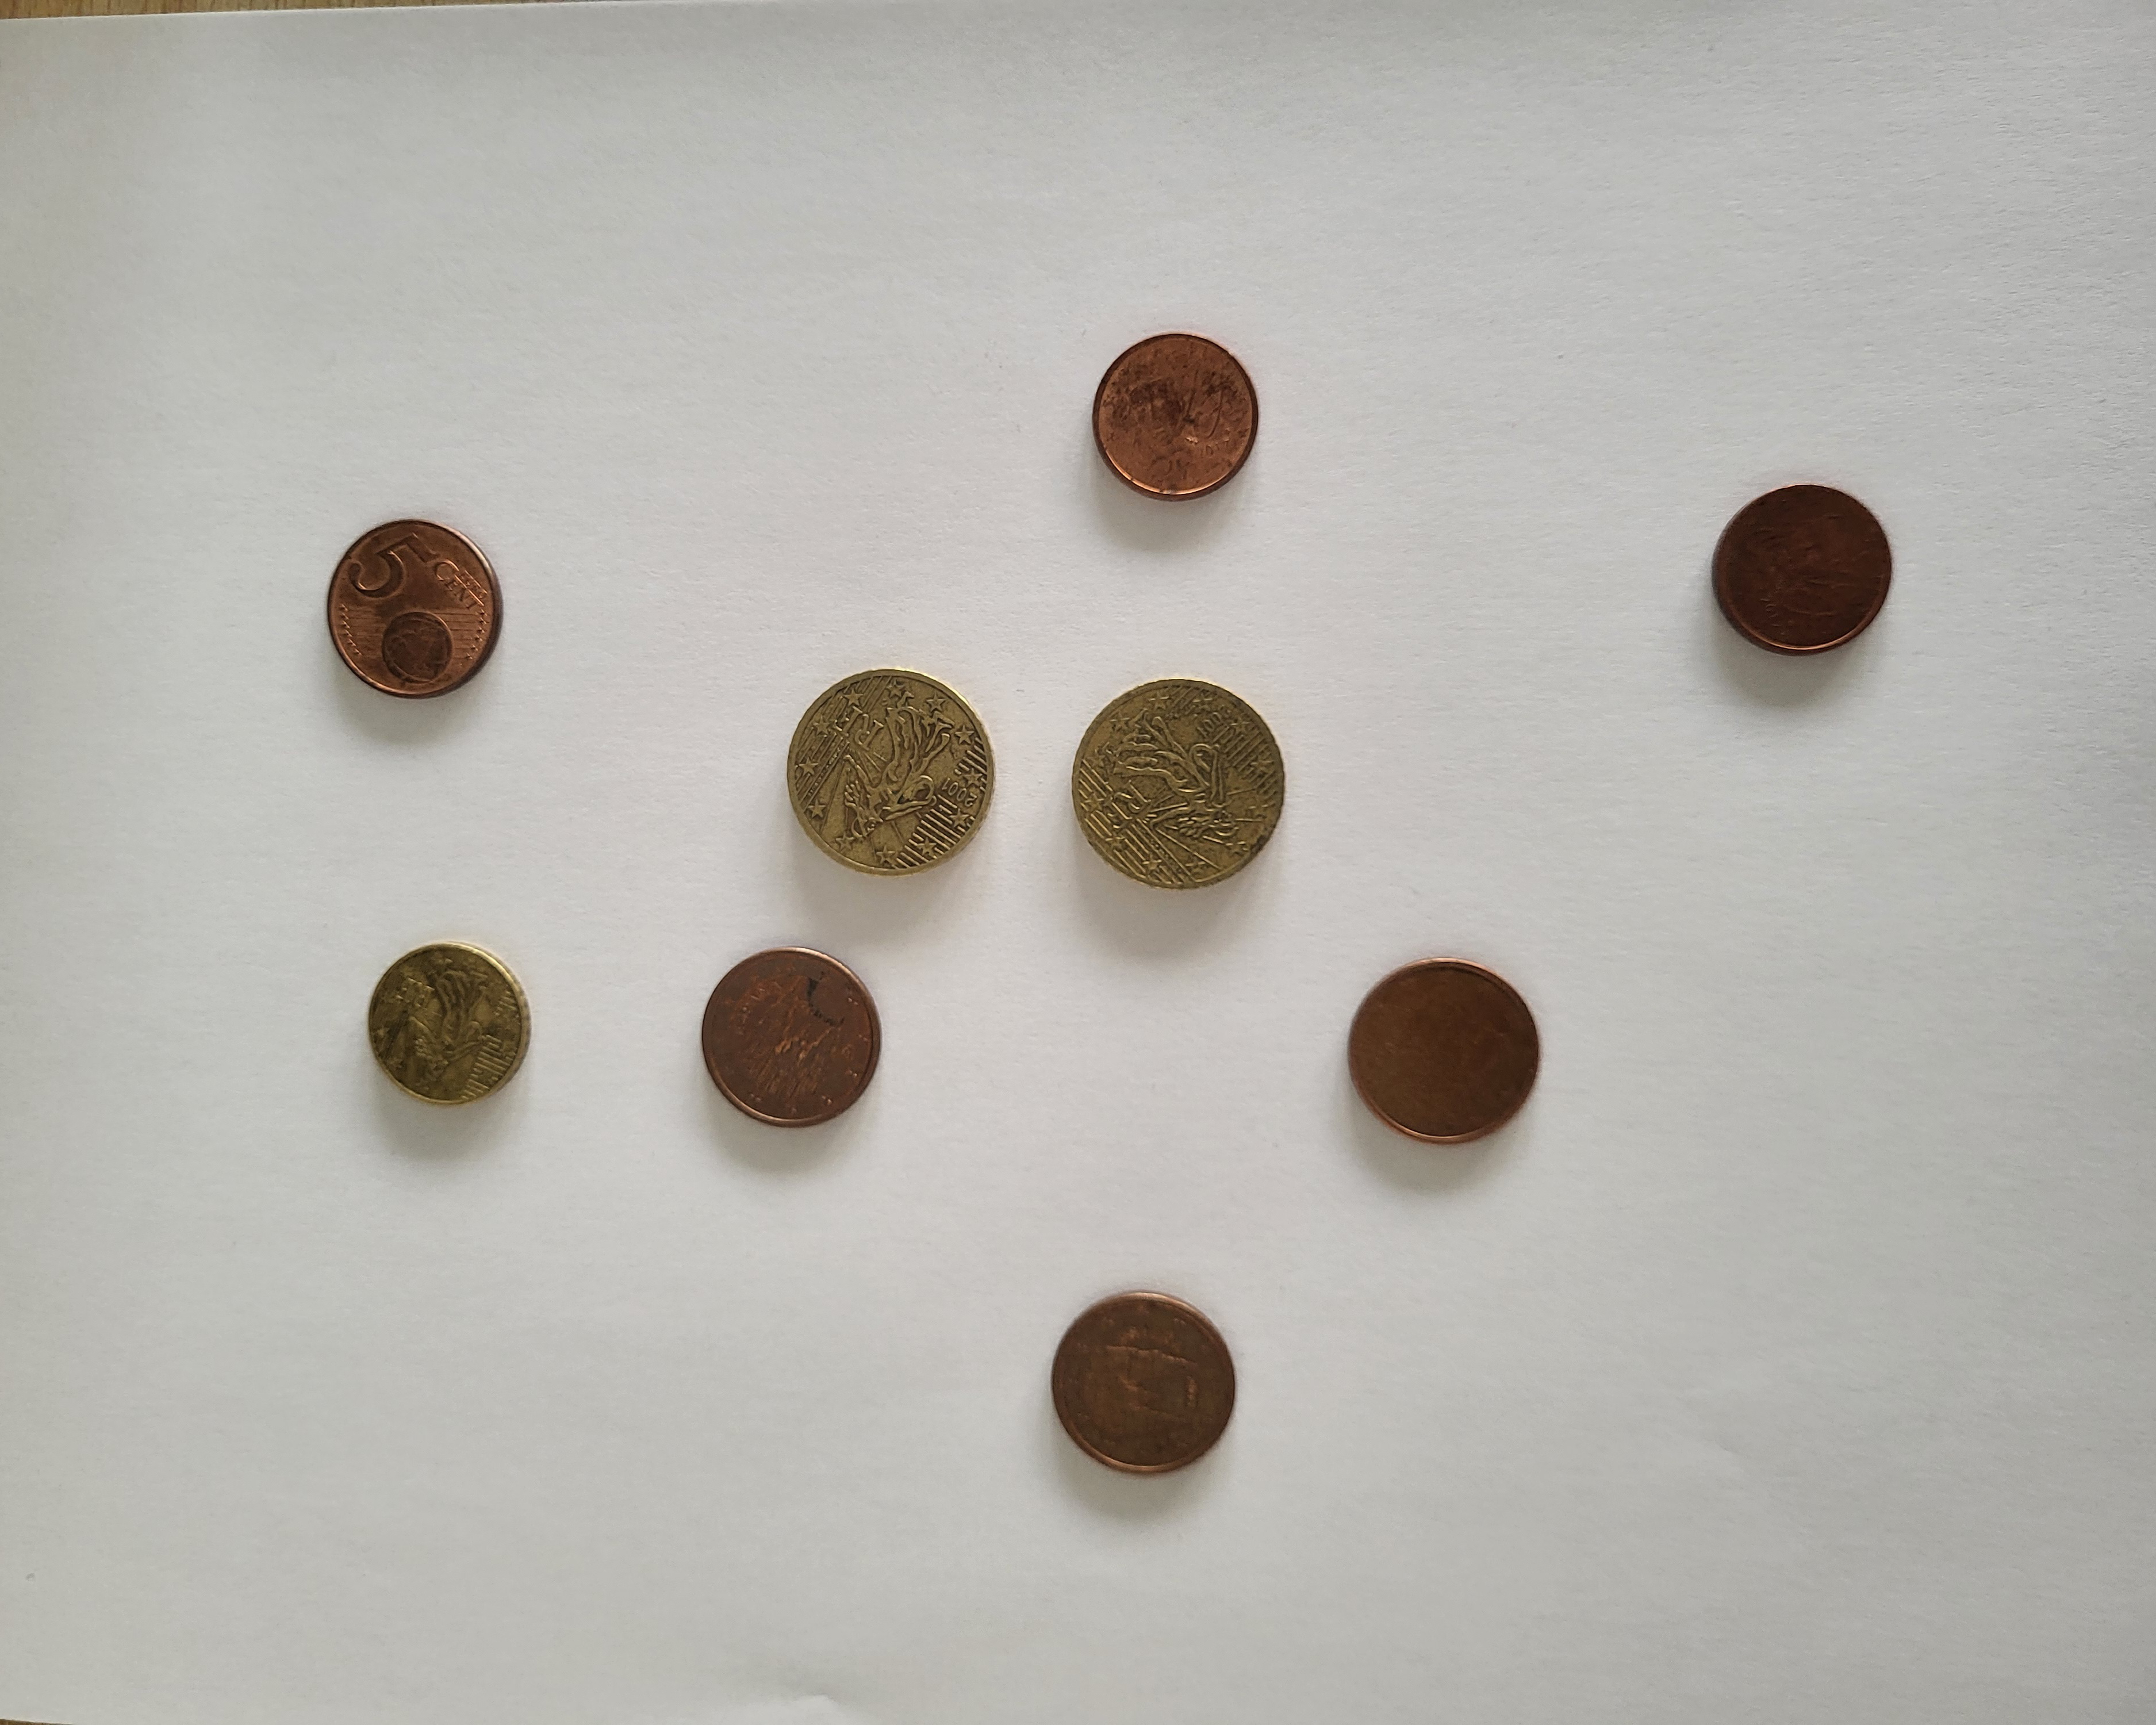
\includegraphics[width=0.5\textwidth]{./object/g1.jpeg}
			\caption{Spectre du signal avec harmoniques $3$ et $5$ supprimées}
		}

		\ffigbox{
			\includegraphics[width=0.5\textwidth]{./object/g2.jpeg}
			\caption{Chronogramme du signal de commande $v_c(t)$}
		}

	\end{floatrow}
\end{figure}



On obtient comme nous le voulions un spectre dont les harmoniques de rang 3 et 5 ont été supprimés et un signal de commmande conforme à ce qui à été trouvé lors de la pré-étude.




















\end{document}
